\chapter{Conclusion}
\renewcommand{\baselinestretch}{\mystretch}
\label{chap:Conclu}
%\setlength{\parindent}{0pt}

\section{Contribution to 3D printing in space}
In this project, the main work is applying lunar and martian dust simulants for the entire FDM technique, including the manufacture of the printable filament and the 3D printing of microscope components. The key challenges are the combination of ABS pellets, pumice powder and the investigation of the filament printability. The solution to the first problem is slightly melting the ABS pellets so the very fine pumice powder can uniform lyattached to their surface. Then the sufficient mixture is processed by the screw of the extruder. The finding of the latter one is that the filament made of 1 wt.\%- 7 wt.\% could be printable in UM2 with the settings of 240$^{\circ}$C extruding temperature without fans, 105$^{\circ}$C build plate with PVA based glue and a relatively low print speed. In particular, a small quantity of pumice powder could improve the printability of ABS based filament. This finding offers the potential that Lunar and Mars dust could be applied as a raw material for FDM technique. 

\section{Limitations of this project}
The findings of this study are restricted to the unprofessional equipments. The printability of the filament could be better if the extruder works better. The lack of the mechanical test of the 3D-printed waveguides means that we cannot recognize the influence of the pumice powder on the prints and the value of the 3D-printed waveguides clearly. \\
\\
There is no accurate data representing how much pumice contained in the filament. Therefore, our experiment is a guess work that demonstrates the possibility of using Lunar/Mars Dust simulants in the FDM system.

\section{Future work}

\subsection{The utilisation of Topas polymers as the base material}
This study has addressed only the combination of ABS pellets and Lunar/Mars dust simulants. There is another interesting material called Topas polymers (8007S-04, TOPAS Advanced Polymer Co.). This material has a tricky property that it is softer than ABS at its glass transition temperature (i.e. 78$^{\circ}$C). Due to this mechanical property, the extruder Noztek Pro seems not very suitable for Topas filament manufacturing as the diameter could have a quite big tolerance. The extruded Topas filament by Noetek Pro extruder could be seen in Figure \ref{Fig:Topaz polymer} below. Its diameter is not uniform, which varies from 2.35mm to 2.78mm with 180$^{\circ}$C extruding temperature specifically. The Topas filament stretches a lot when it goes through the filament guiding gate of the extruder. It is highly certain that this kind of polymers could produce a printable filament with other extruder or equipment. \\
\\
The outstanding property of it is the transparent colour which is an ideal material to produce the optical components. And there is a strong possibility of the combination of Topas and Lunar/Mars dust since Topas polymers are sticky at high temperature while the latter increases the brittleness of the filament.  
\begin{figure}[htbp]
  \centering
  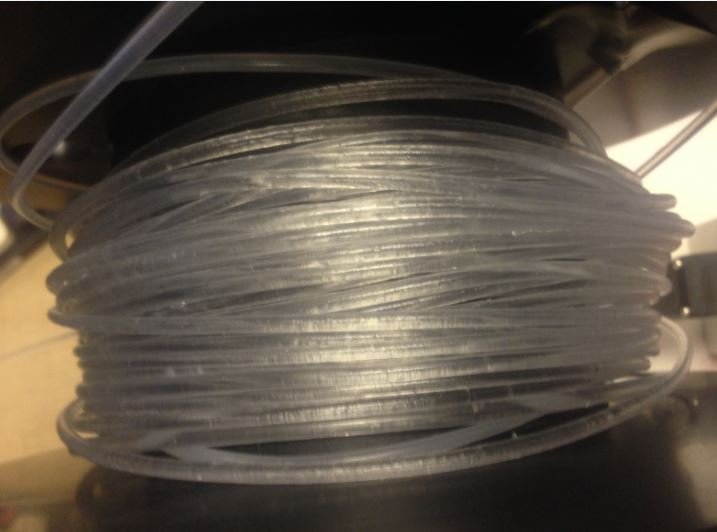
\includegraphics[scale=0.5]{Figs5//topaz_filament.JPG}
  \caption[The Topas filament]{\footnotesize The Topas filament.}
  \label{Fig:Topaz polymer}
\end{figure}

\subsection{The restriction of using ABS with Lunar and Mars regolith}
It seems the blends of ABS and Lunar/Mars regolith have some limitations for FDM technique. The brittleness of the filament made of the blends could cause the failure of printing. There is a strong possibility to add some material to make it soft and sticky at extruding temperature or use other thermoplastics to mix with the blends of ABS and Lunar/Mars dust simulants. This material might decrease the brittleness of the mixture so that the proportion of Lunar/Mars dust could be increased.
